This experiment is to test how static and dynamic memory allocation of Java and Rust behave. For the assessment, Element addition to ArrayList in the case of Java and Vector in the case of Rust 
is emploied here. These data stractures are resizable and we have control to set initial size. There are two parameters; initial size of ArrayList or Vector and thier final size after additions of elements. 
We are interested in the impact to runtime performance by initializing memory allocation and dynamicaly allocating memory space.

First, an ArrayList and an Vector are created with specified initial size. Then, in a loop, a element is added for each iteration until the size of the ArrayList or Vector get the specified final size. 
Each data structure has a different resizing strategy. When an ArrayList hits current limit of its size and expands the limit, it doubles the current size.  
While Vector does not have specific strategy for its resizing, the expantions of size of both ArrayList and Vector might affect the digradation of runtime performance.

Second, four types of element are used for elements addition to each data structure: integer, array of charactors, string, and Customer object. 
Assamption is that there would be different behavior between element additions of dynamically resizable and static size objects. 
Customer object has three fields. These fields are total order, weight of order, and zip code whose types are integer (i32 in rust), double (f32 in rust), and string respectively.
Figure 2-6 and 2-7 are representations of customer objects in Java and Rust.

Figure 2-10, 2-11, 2-12, and 2-13 represent the result of the experiments. For both data structures, integer elements addition shows the fastest runtime among all object types. 
This is because the compilers know each integer need 4 bytes to be stored in memory so that the space for memory that should be allocated is easily inspected. 
For the same reason, the initialization of data structures whose elements are integers alaways improves runtim performance.

The elements addition of strings and array of character behave similally among each languages. These two types of elements addition perform the similar speed and significantly slower than integer addition. 
Customer object addition is the slowest in Java. However, in Rust the addition of Customer object is the second fastest among all element typs.
The impacts of initialization of Java ArrayList vary among elemet types. On the other hand, the initailization Rust Vector always improves runtime performance for any of 4 types of elements addition.


\begin{figure}[htb]
    \begin{lstlisting}[
            basicstyle=\tiny, %or \small or \footnotesize etc.
        ]
        class Customer {
            int totalOrder;
            double weightOrder;
            String zipCode;
        }
    \end{lstlisting}
    \caption{Representation of Customer object in Java.}
    \label{fig:Sampling}    
\end{figure}

\begin{figure}[htb]
    \begin{lstlisting}[
            basicstyle=\tiny, %or \small or \footnotesize etc.
        ]
        struct Customer {
            total_order: i32,
            weight_order: f32,
            zip_code: String,
        }
    \end{lstlisting}
    \caption{Representation of Customer object in Rust.}
    \label{fig:Sampling}
\end{figure}

\begin{figure}[htb]
    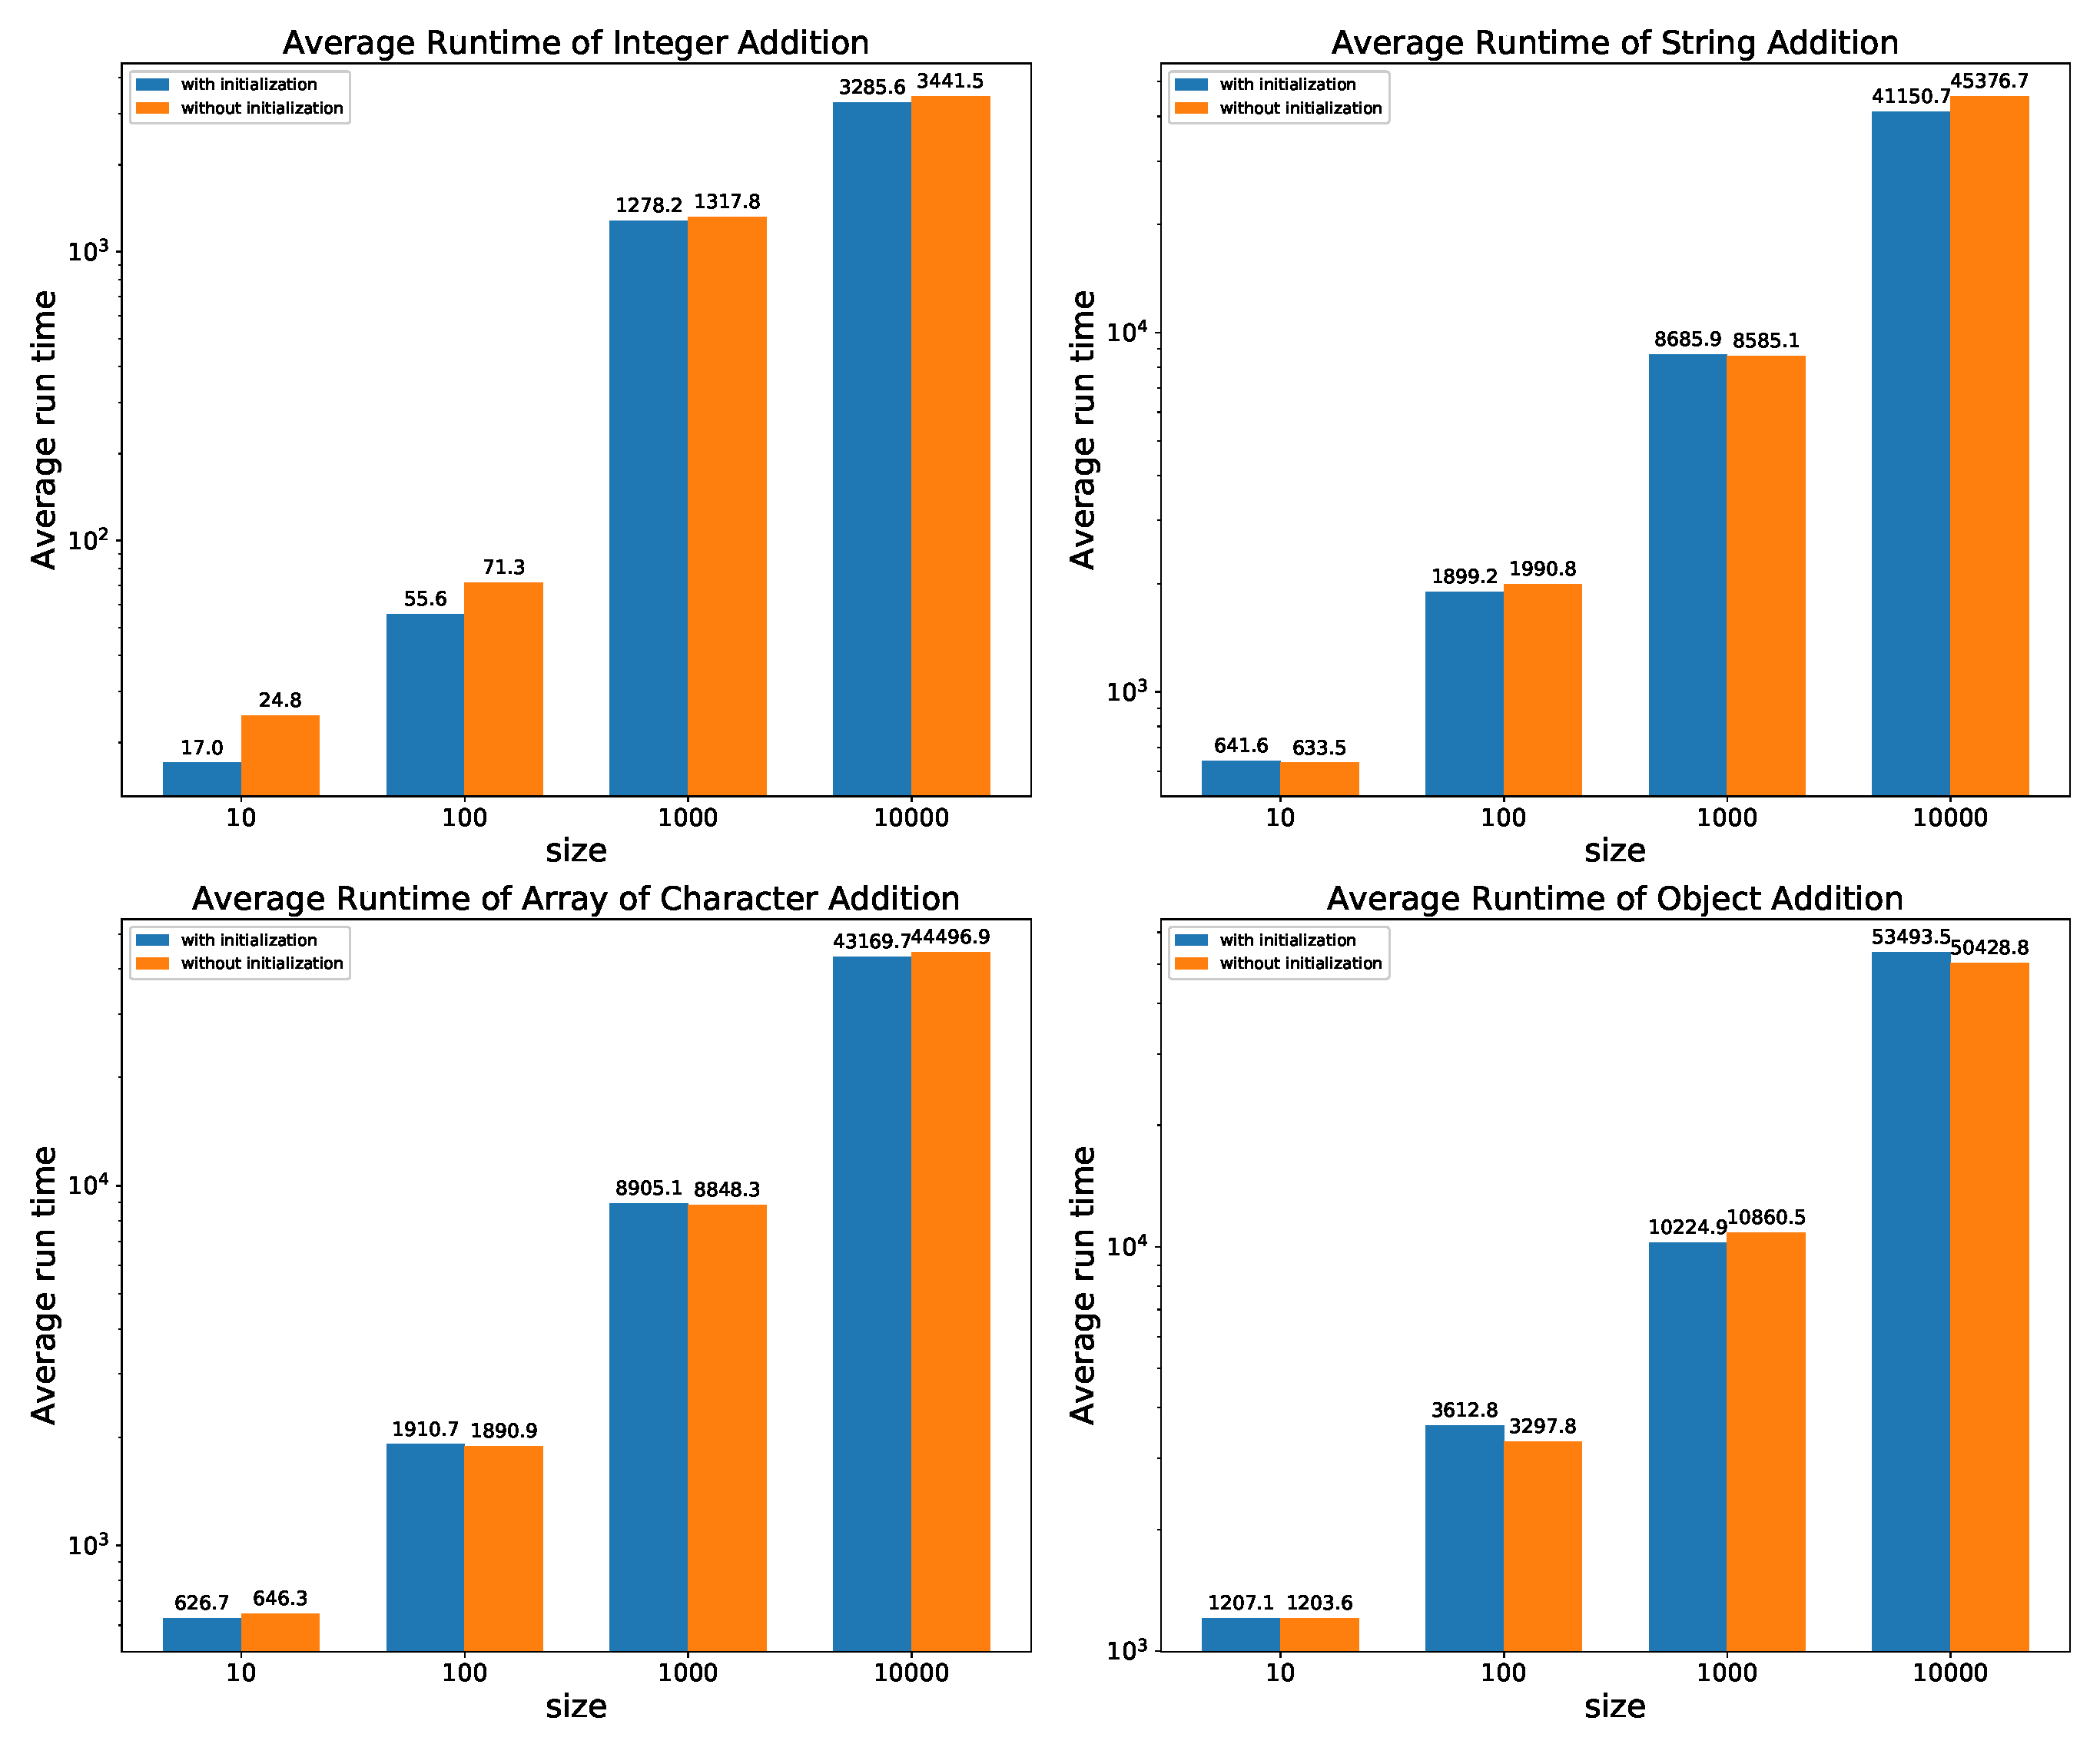
\includegraphics[width=15cm]{java_arraylist_log.eps}
    \caption{Memory allocation of Java ArrayList}
    \label{fig:Sampling}
\end{figure}

\begin{figure}[htb]
    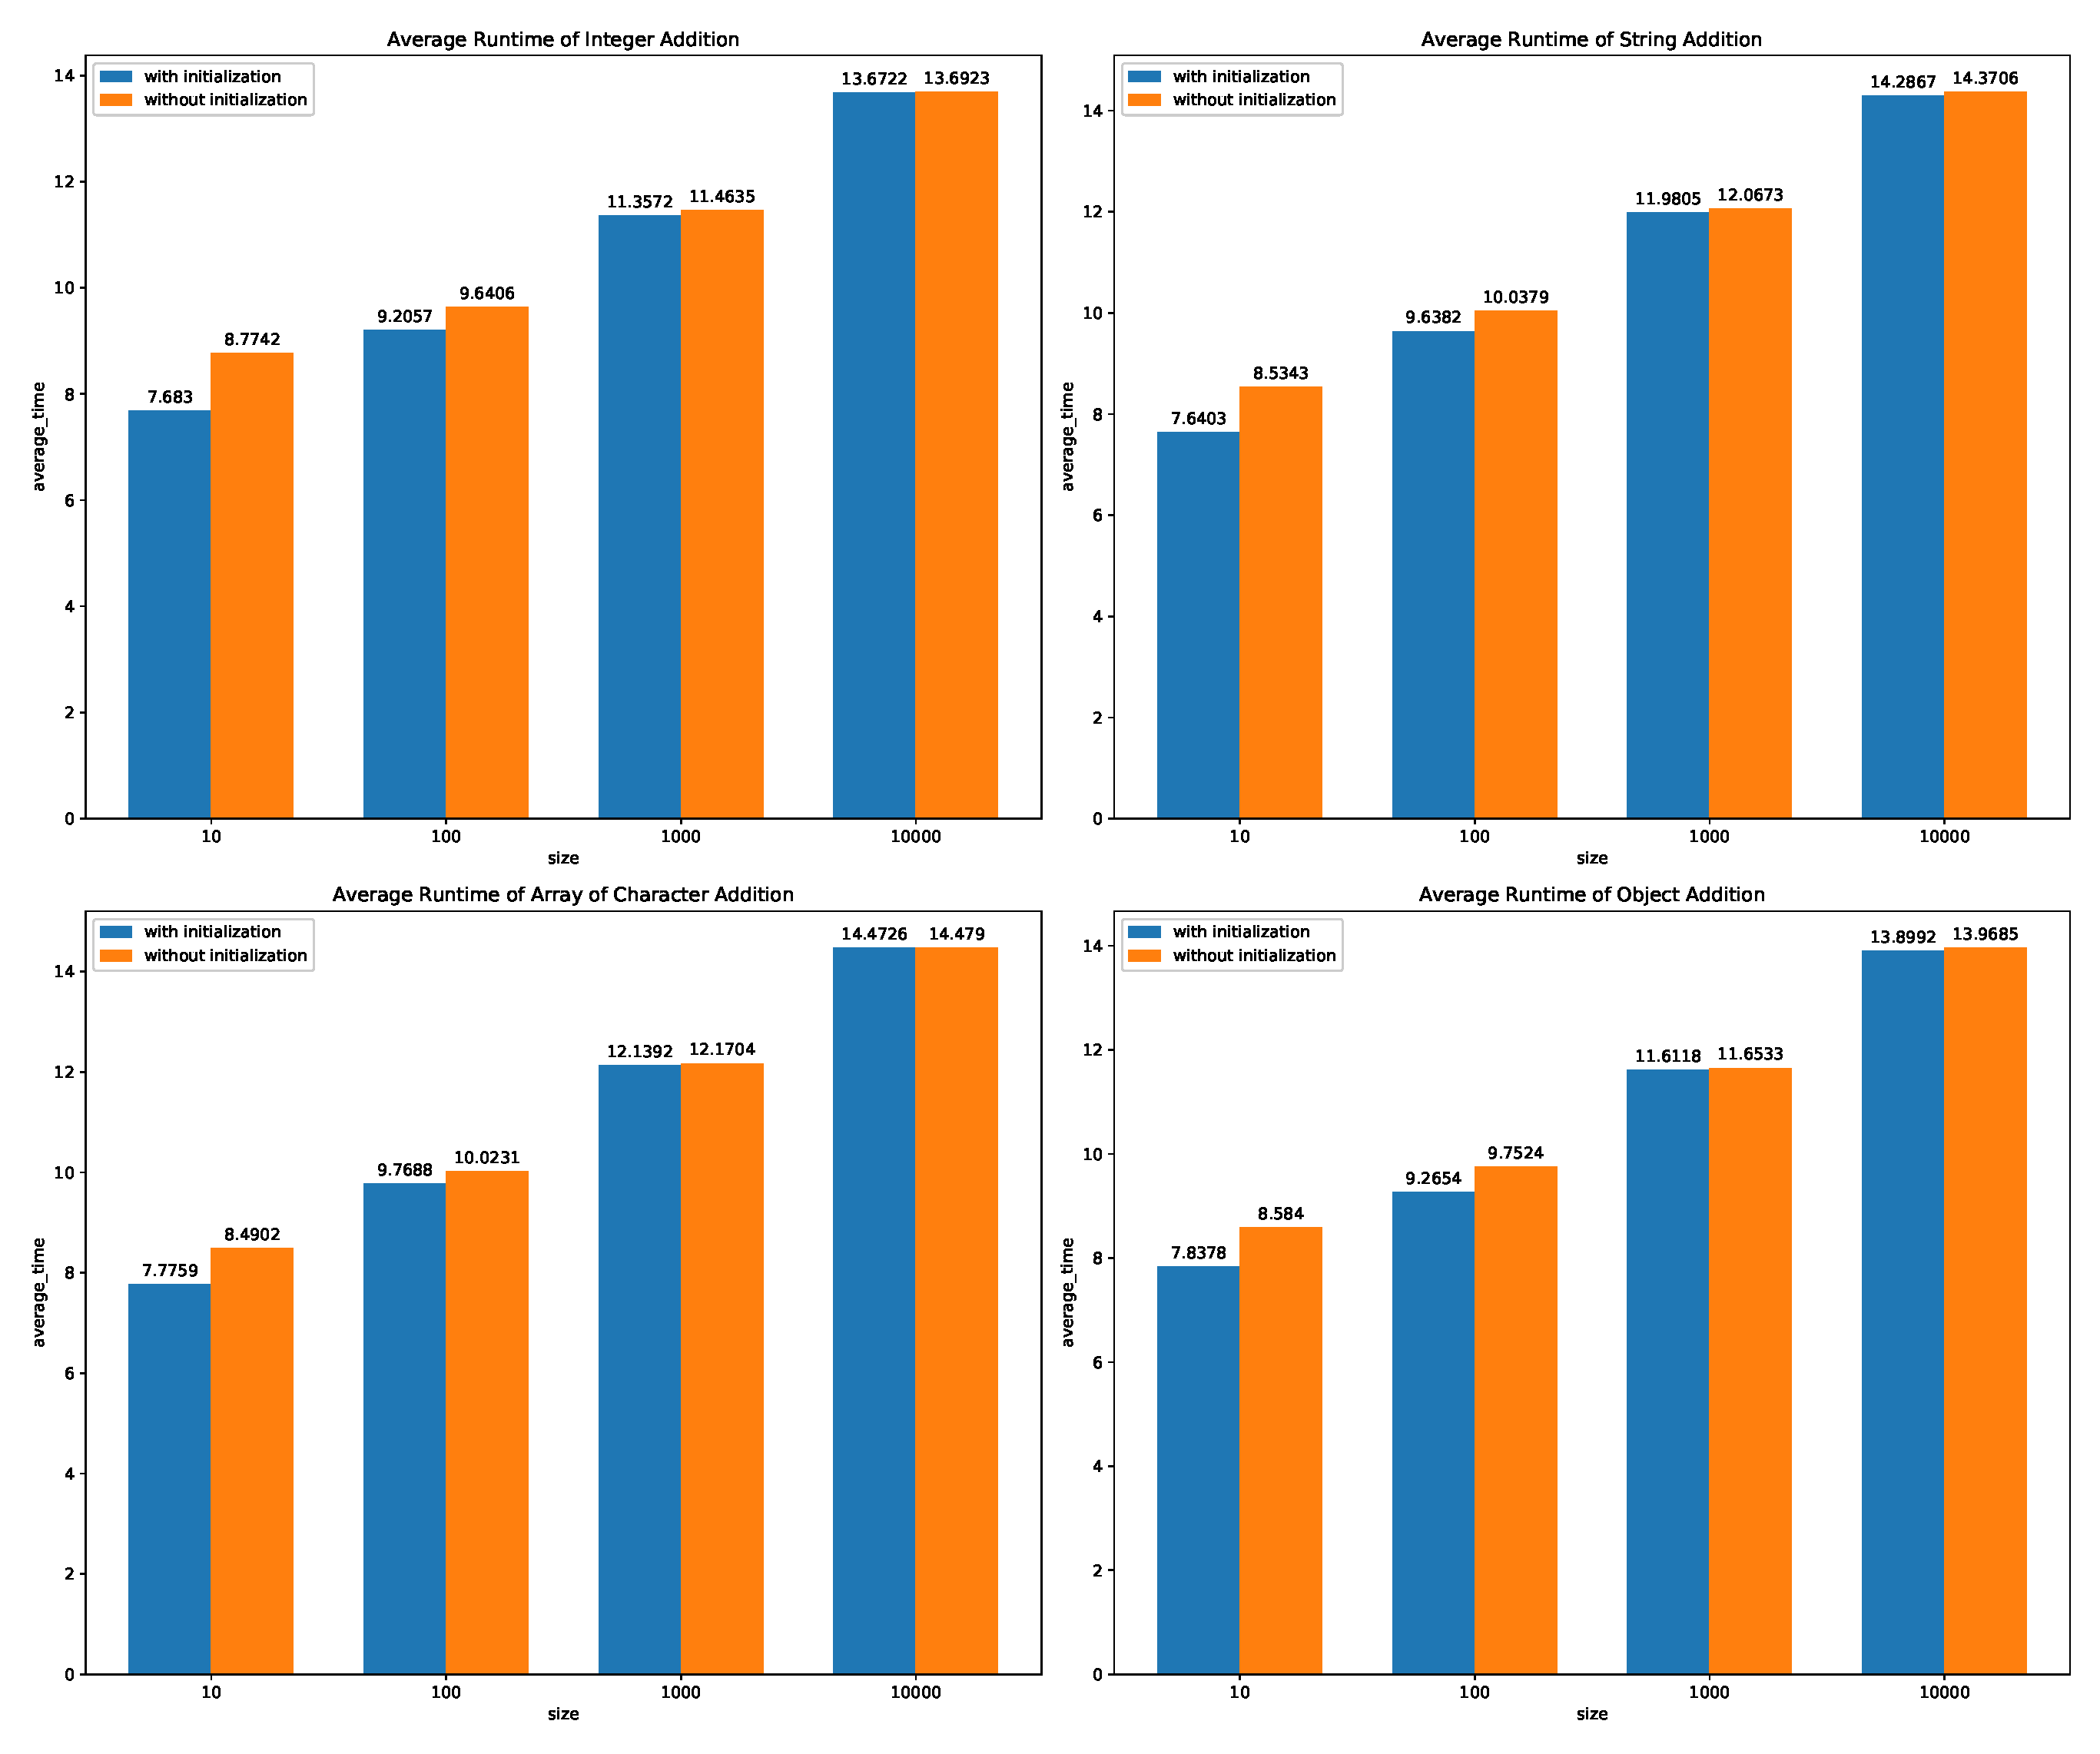
\includegraphics[width=15cm]{rust_vector_log.eps}
    \caption{Memory allocation of Rust Vector}
    \label{fig:Sampling}
\end{figure}


\begin{figure}[htb]
    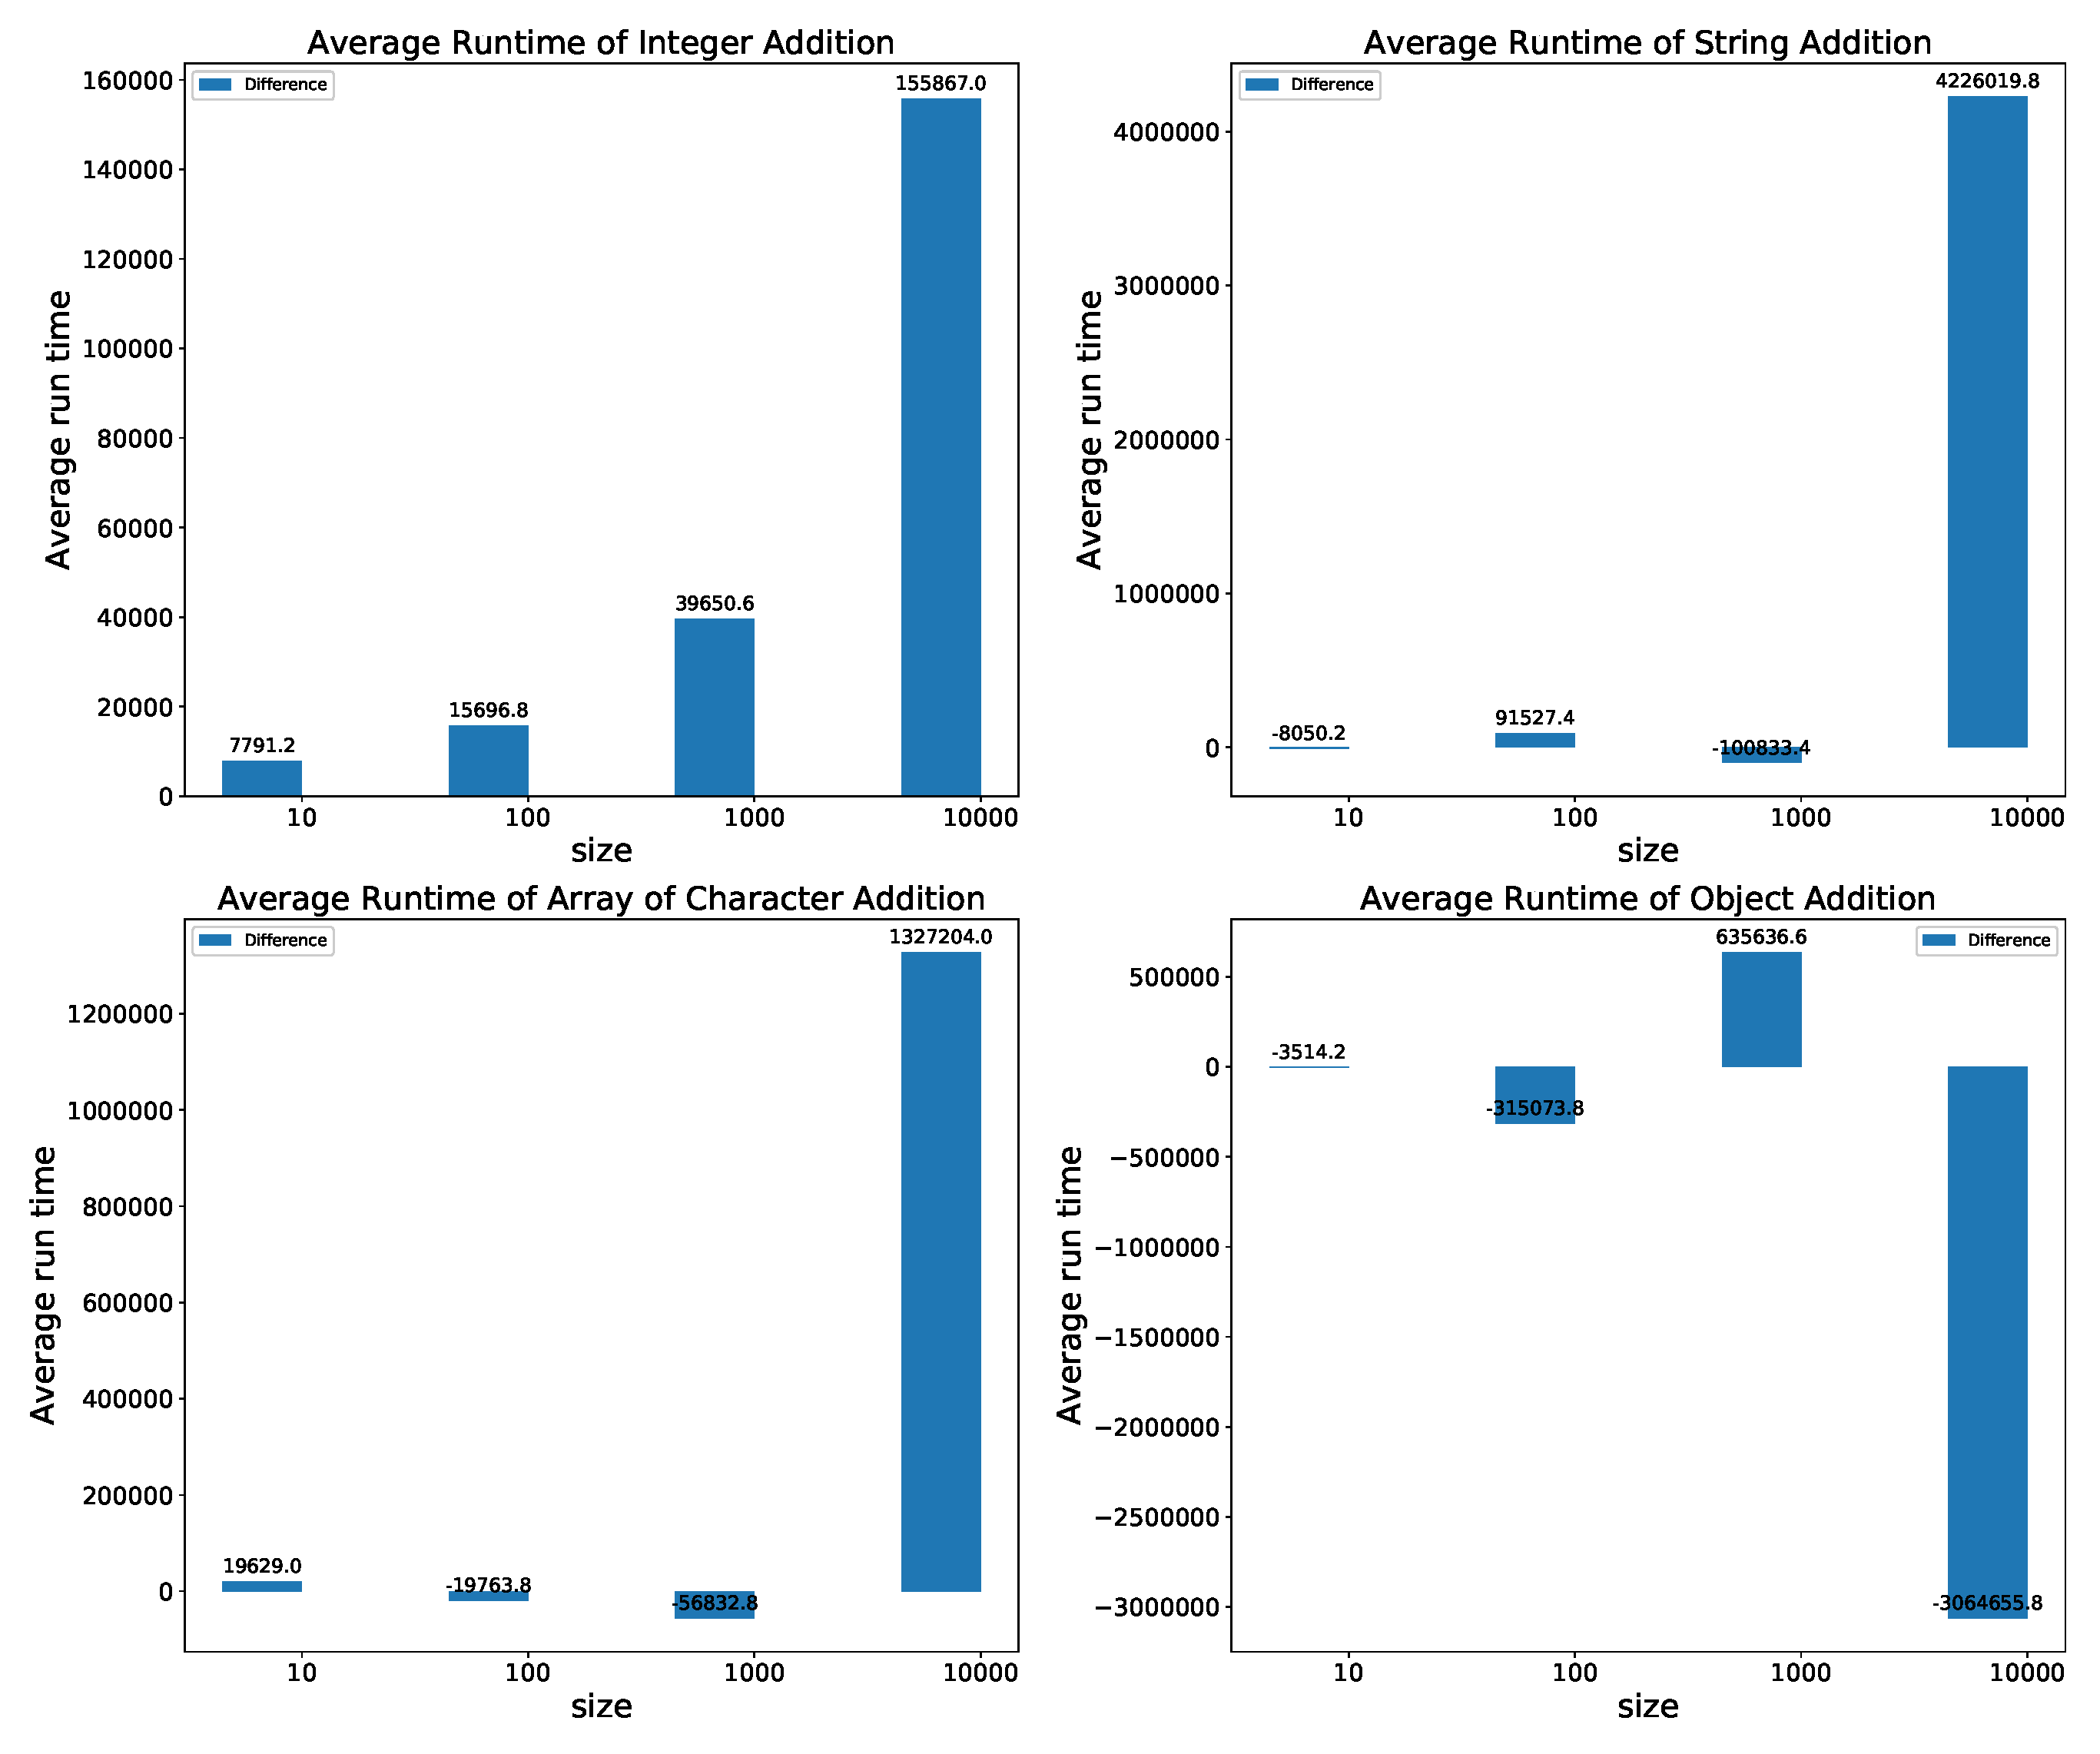
\includegraphics[width=15cm]{java_arraylist_difference.eps}
    \caption{Difference of Memory allocation of Java ArrayList between Non-initialization and Initialization}
    \label{fig:Sampling}
\end{figure}

\begin{figure}[htb]
    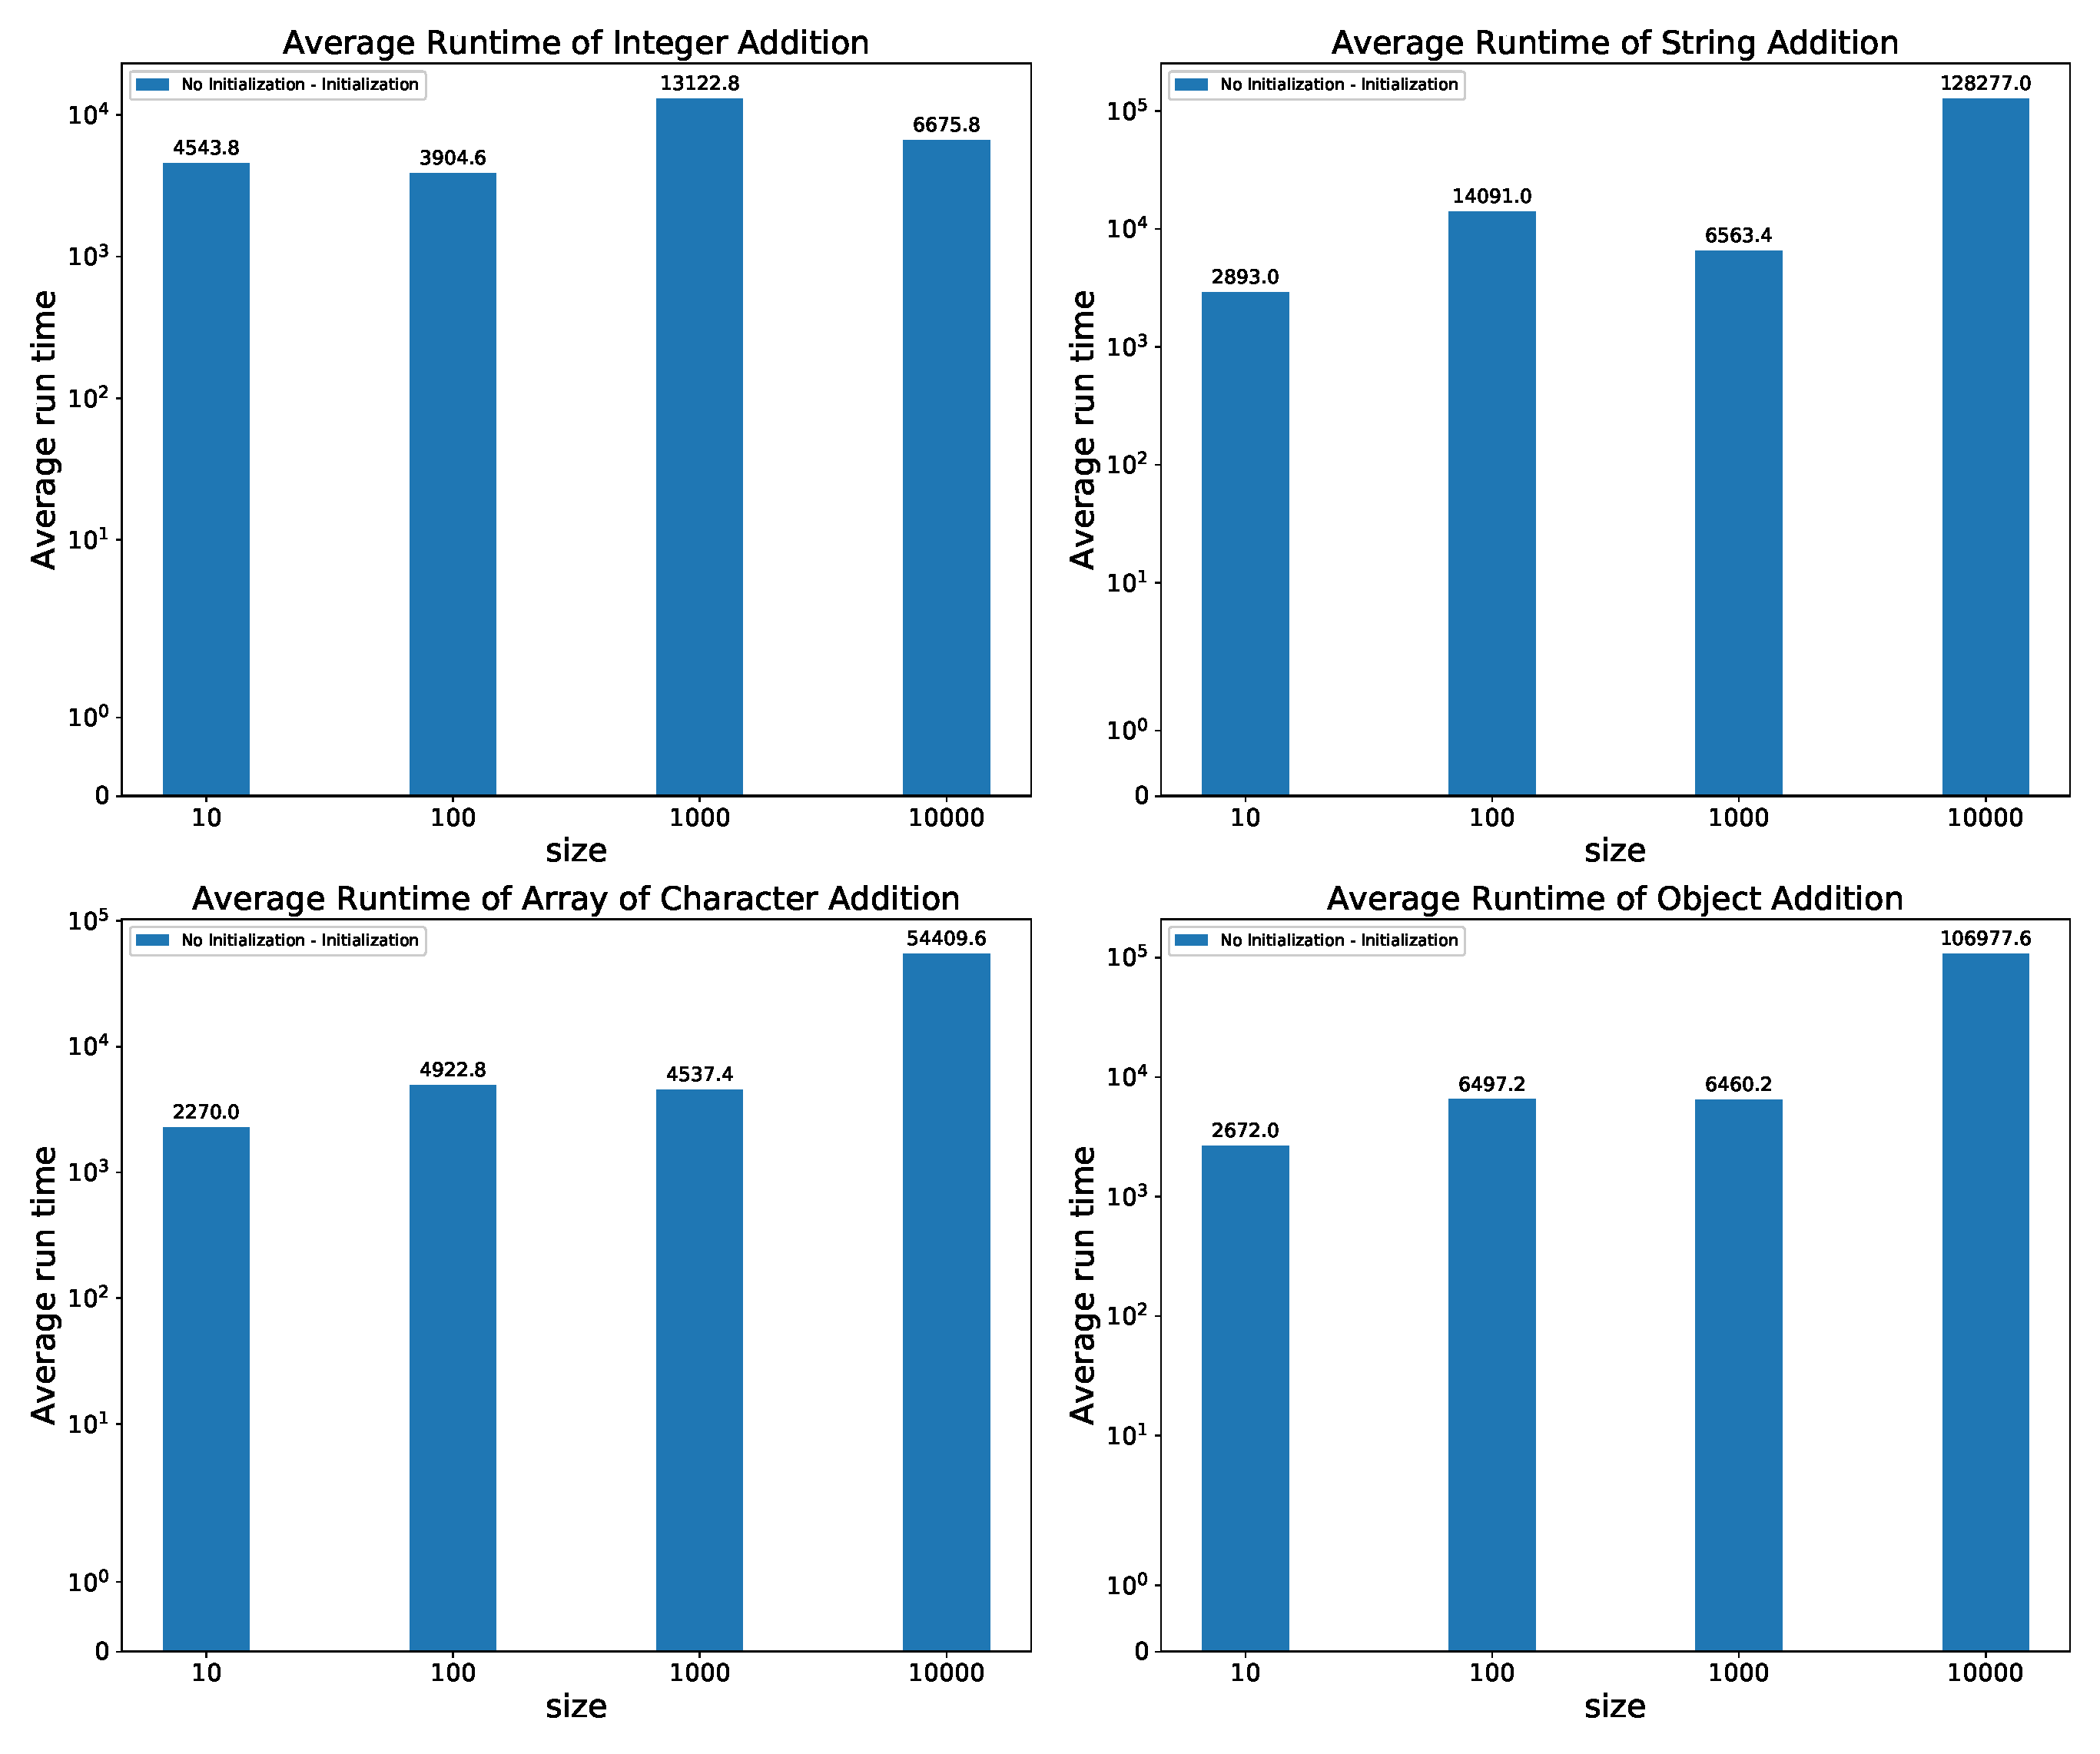
\includegraphics[width=15cm]{rust_arraylist_difference.eps}
    \caption{Difference of Memory allocation of Rust Vector between Non-initialization and Initialization}
    \label{fig:Sampling}
\end{figure}